% Standalone GINE architecture figure for the traffic-scene graph embedding model.
% Compile with: pdflatex graph_gine_architecture_tikz.tex
% Produces graph_gine_architecture_tikz.pdf, which is included by
% sections_safecomp/07_create_graph_embeddings.tex
\documentclass[border=4pt]{standalone}
\usepackage[T1]{fontenc}
\usepackage{amsmath}
\usepackage{amssymb}
\usepackage{xcolor}
\usepackage{tikz}
\usetikzlibrary{positioning,arrows.meta,fit,backgrounds,calc,shapes.geometric,fadings}

% ---- colour palette (muted, print friendly) -------------------------------
\definecolor{cInput}{HTML}{E8EEF7}
\definecolor{cInputB}{HTML}{4C72B0}
\definecolor{cConv}{HTML}{DCE9F5}
\definecolor{cConvB}{HTML}{2F6FB0}
\definecolor{cPool}{HTML}{E3F0E1}
\definecolor{cPoolB}{HTML}{3F8A3F}
\definecolor{cHead}{HTML}{FBE9D8}
\definecolor{cHeadB}{HTML}{D77B2A}
\definecolor{cLoss}{HTML}{F8E0E0}
\definecolor{cLossB}{HTML}{C0392B}
\definecolor{cAug}{HTML}{EDE6F4}
\definecolor{cAugB}{HTML}{7E57A8}
\definecolor{cGroup}{HTML}{F7F7F9}

\begin{document}
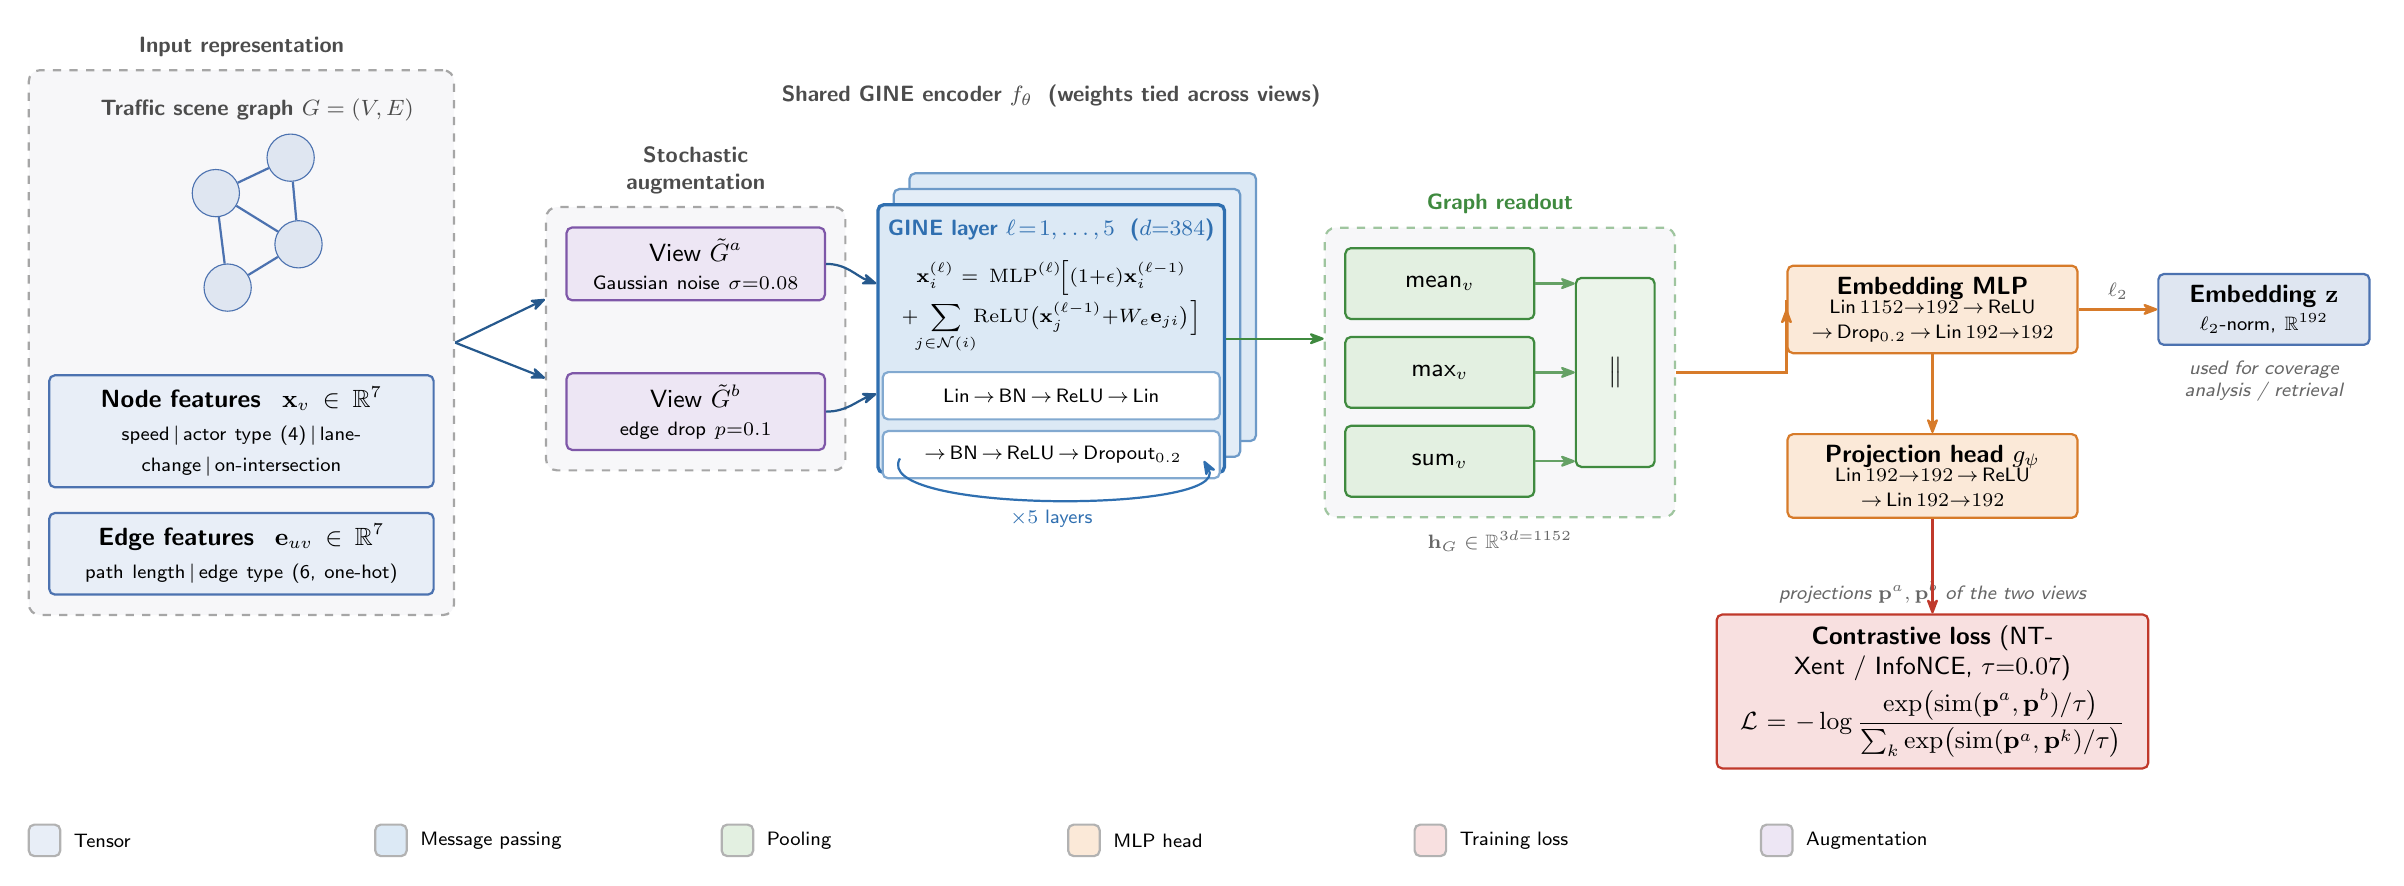
\begin{tikzpicture}[
  font=\sffamily\small,
  >={Stealth[round]},
  node distance=6mm,
  block/.style={rounded corners=2pt,draw,thick,align=center,inner sep=4pt,minimum height=9mm},
  io/.style    ={block,fill=cInput,draw=cInputB},
  conv/.style  ={block,fill=cConv,draw=cConvB},
  pool/.style  ={block,fill=cPool,draw=cPoolB},
  head/.style  ={block,fill=cHead,draw=cHeadB},
  loss/.style  ={block,fill=cLoss,draw=cLossB},
  aug/.style   ={block,fill=cAug,draw=cAugB},
  flow/.style  ={->,thick,cConvB!80!black},
  dimlab/.style={font=\sffamily\scriptsize\itshape,text=black!60},
  grp/.style   ={rounded corners=4pt,draw=black!35,dashed,thick,fill=cGroup,inner sep=7pt},
  grptitle/.style={font=\sffamily\bfseries\footnotesize,text=black!70},
]

% =====================================================================
% (A)  INPUT : traffic scene graph + feature decomposition
% =====================================================================
% --- little scene graph drawing -------------------------------------------------
\begin{scope}[local bounding box=GRAPH]
  \node[circle,draw=cInputB,fill=cInputB!18,minimum size=6mm,inner sep=0] (n1) at (0,0.55)  {};
  \node[circle,draw=cInputB,fill=cInputB!18,minimum size=6mm,inner sep=0] (n2) at (0.95,1.0){};
  \node[circle,draw=cInputB,fill=cInputB!18,minimum size=6mm,inner sep=0] (n3) at (1.05,-0.1){};
  \node[circle,draw=cInputB,fill=cInputB!18,minimum size=6mm,inner sep=0] (n4) at (0.15,-0.65){};
  \foreach \a/\b in {n1/n2,n1/n3,n3/n4,n2/n3,n1/n4}
     \draw[cInputB,thick] (\a) -- (\b);
\end{scope}
\node[grptitle,above=1pt of GRAPH] (gtitle) {Traffic scene graph $G=(V,E)$};

% --- node-feature token ----------------------------------------------------------
\node[io,below=8mm of GRAPH.south,xshift=-2mm,text width=46mm] (xfeat)
  {\textbf{Node features} $\;\mathbf{x}_v\in\mathbb{R}^{7}$\\[1pt]
   \scriptsize speed\,$\mid$\,actor type (4)\,$\mid$\,lane-change\,$\mid$\,on-intersection};
% --- edge-feature token ----------------------------------------------------------
\node[io,below=3mm of xfeat,text width=46mm] (efeat)
  {\textbf{Edge features} $\;\mathbf{e}_{uv}\in\mathbb{R}^{7}$\\[1pt]
   \scriptsize path length\,$\mid$\,edge type (6, one-hot)};

% group box for the whole input column
\begin{scope}[on background layer]
  \node[grp,fit=(gtitle)(GRAPH)(xfeat)(efeat)] (INPUT) {};
\end{scope}
\node[grptitle,above=1pt of INPUT.north] {Input representation};

% =====================================================================
% (B)  AUGMENTATION : two correlated views
% =====================================================================
\node[aug,right=14mm of INPUT.east,yshift=10mm,text width=30mm] (augA)
  {View $\tilde G^{a}$\\[-1pt]\scriptsize Gaussian noise $\sigma{=}0.08$};
\node[aug,below=9mm of augA,text width=30mm] (augB)
  {View $\tilde G^{b}$\\[-1pt]\scriptsize edge drop $p{=}0.1$};
\begin{scope}[on background layer]
  \node[grp,fit=(augA)(augB)] (AUG) {};
\end{scope}
\node[grptitle,above=1pt of AUG.north,align=center] {Stochastic\\augmentation};

\draw[flow] (INPUT.east) -- ($(AUG.west)+(0,5mm)$);
\draw[flow] (INPUT.east) -- ($(AUG.west)-(0,5mm)$);

% =====================================================================
% (C)  SHARED GINE ENCODER  f_theta  (5 stacked layers, one expanded)
% =====================================================================
% stacked-layer look : three offset rectangles behind the detailed one
\coordinate (encanchor) at ($(AUG.east)+(26mm,0)$);
\foreach \i in {2,1}{
  \node[conv,minimum width=44mm,minimum height=34mm,
        fill=cConv!\the\numexpr60+20*\i\relax, draw=cConvB!70,
        anchor=center] at ($(encanchor)+(\i*2mm,\i*2mm)$) {};
}
\node[conv,minimum width=44mm,minimum height=34mm,anchor=center,
      fill=cConv,draw=cConvB,very thick] (ENC) at (encanchor) {};

% header inside the front layer
\node[grptitle,anchor=north,text=cConvB] at ($(ENC.north)+(0,-2pt)$)
  {GINE layer $\ell\!=\!1,\dots,5$ \;($d{=}384$)};

% message passing equation
\node[align=center,font=\sffamily\scriptsize,anchor=north,text width=42mm]
  at ($(ENC.north)+(0,-6mm)$) (mpeq)
  {$\displaystyle \mathbf{x}_i^{(\ell)}\!=\mathrm{MLP}^{(\ell)}\!\Big[(1{+}\epsilon)\mathbf{x}_i^{(\ell-1)}$\\[1pt]
   $\displaystyle +\!\!\sum_{j\in\mathcal{N}(i)}\!\!\mathrm{ReLU}\big(\mathbf{x}_j^{(\ell-1)}{+}W_e\mathbf{e}_{ji}\big)\Big]$};

% the per-layer MLP internals as a mini pipeline
\node[block,fill=white,draw=cConvB!60,font=\sffamily\scriptsize,
      anchor=north,minimum height=6mm,text width=40mm]
      at ($(mpeq.south)+(0,-1mm)$) (mlp)
  {Lin\,$\to$\,BN\,$\to$\,ReLU\,$\to$\,Lin};
\node[block,fill=white,draw=cConvB!60,font=\sffamily\scriptsize,
      anchor=north,minimum height=6mm,text width=40mm,below=1.2mm of mlp] (post)
  {\,$\to$\,BN\,$\to$\,ReLU\,$\to$\,Dropout$_{0.2}$};

% encoder group label
\node[grptitle,above=11mm of ENC.north,align=center]
  {Shared GINE encoder $f_\theta$ \;(weights tied across views)};

% augmented views feed encoder
\draw[flow] (augA.east) to[out=0,in=160] ($(ENC.west)+(0,7mm)$);
\draw[flow] (augB.east) to[out=0,in=200] ($(ENC.west)-(0,7mm)$);
% recurrence arrow (xN)
\draw[->,thick,cConvB,shorten >=1pt]
  ($(ENC.south west)+(3mm,2mm)$) .. controls +(-4mm,-7mm) and +(4mm,-7mm) ..
  ($(ENC.south east)+(-3mm,2mm)$)
  node[midway,below,font=\sffamily\scriptsize,text=cConvB]{$\times 5$ layers};

% =====================================================================
% (D)  READOUT : multi pooling -> concat
% =====================================================================
\node[pool,right=15mm of ENC.east,yshift=7mm,minimum width=24mm] (pmean){mean$_v$};
\node[pool,below=2mm of pmean,minimum width=24mm] (pmax){max$_v$};
\node[pool,below=2mm of pmax,minimum width=24mm] (psum){sum$_v$};
\node[pool,right=5mm of pmax,minimum width=10mm,minimum height=24mm,
      fill=cPool!70] (concat){$\big\|$};
\begin{scope}[on background layer]
  \node[grp,fit=(pmean)(pmax)(psum)(concat),draw=cPoolB!50] (POOL){};
\end{scope}
\node[grptitle,above=1pt of POOL.north,text=cPoolB,align=center]
  {Graph readout};
\node[dimlab,below=1pt of POOL.south]{$\mathbf{h}_G\in\mathbb{R}^{3d=1152}$};

\draw[flow,cPoolB] (ENC.east) -- (POOL.west|-ENC.east);
\foreach \p in {pmean,pmax,psum}\draw[->,thick,cPoolB!80] (\p.east)--(\p.east-|concat.west);

% =====================================================================
% (E)  HEADS : embedding MLP (downstream) + projection head (training)
% =====================================================================
\node[head,right=14mm of POOL.east,yshift=8mm,text width=34mm] (emb)
  {\textbf{Embedding MLP}\\[-1pt]\scriptsize Lin\,$1152{\to}192$\,$\to$\,ReLU\\[-2pt]
   \scriptsize $\to$\,Drop$_{0.2}$\,$\to$\,Lin\,$192{\to}192$};
\node[head,below=10mm of emb,text width=34mm] (proj)
  {\textbf{Projection head} $g_\psi$\\[-1pt]\scriptsize Lin\,$192{\to}192$\,$\to$\,ReLU\\[-2pt]
   \scriptsize $\to$\,Lin\,$192{\to}192$};

% normalized embedding output (the one actually used downstream)
\node[io,right=10mm of emb,fill=cInputB!18,draw=cInputB,text width=24mm] (zout)
  {\textbf{Embedding} $\mathbf{z}$\\[-1pt]\scriptsize $\ell_2$-norm, $\mathbb{R}^{192}$};
\node[dimlab,below=2pt of zout,text width=26mm,align=center]
  {used for coverage\\ analysis / retrieval};

\draw[flow,cHeadB] (POOL.east) -- (POOL.east-|emb.west) |- (emb.west);
\draw[flow,cHeadB] (emb.east) -- node[above,dimlab]{$\ell_2$} (zout.west);
\draw[flow,cHeadB] (emb.south) -- (proj.north);

% =====================================================================
% (F)  CONTRASTIVE LOSS (NT-Xent / InfoNCE)
% =====================================================================
\node[loss,below=12mm of proj,text width=52mm] (loss)
  {\textbf{Contrastive loss} (NT-Xent / InfoNCE, $\tau{=}0.07$)\\[2pt]
   $\displaystyle \mathcal{L}= -\log\frac{\exp\!\big(\mathrm{sim}(\mathbf{p}^{a},\mathbf{p}^{b})/\tau\big)}
   {\sum_{k}\exp\!\big(\mathrm{sim}(\mathbf{p}^{a},\mathbf{p}^{k})/\tau\big)}$};
\node[dimlab,above=0pt of loss.north]{projections $\mathbf{p}^{a},\mathbf{p}^{b}$ of the two views};

\draw[flow,cLossB] (proj.south) -- (proj.south|-loss.north);

% =====================================================================
% LEGEND
% =====================================================================
\begin{scope}[shift={($(INPUT.south west |- loss.south)+(0,-9mm)$)},x=1mm,y=1mm]
  \foreach \c/\t [count=\k from 0] in
     {cInput/Tensor / I/O, cConv/Message passing, cPool/Pooling,
      cHead/MLP head, cLoss/Training loss, cAug/Augmentation}{
     \node[block,fill=\c,draw=black!30,minimum width=4mm,minimum height=4mm,
           inner sep=0,anchor=west] (lg) at ({\k*44},0){};
     \node[anchor=west,font=\sffamily\scriptsize,right=1pt of lg]{\t};
  }
\end{scope}

\end{tikzpicture}
\end{document}
